\documentclass[preprint,12pt]{elsarticle}
%% preamble
% preamble.tex

%% packages
\usepackage{times}
\usepackage{amssymb}
\usepackage{amsmath}
\usepackage{theorem}
\usepackage{booktabs}
\usepackage{tabularx}
\usepackage{epstopdf}
\usepackage{flushend}
\usepackage{color}
\usepackage[usenames,dvipsnames,svgnames,table]{xcolor}
\usepackage{algorithm}
\usepackage{algpseudocode}
\usepackage{siunitx}
\usepackage{hyperref}
\usepackage{url}
\usepackage{fixltx2e}
\usepackage{graphicx}
\usepackage{subfigure}
\usepackage{geometry}
\usepackage{supertabular}
\usepackage{bm}
\usepackage{lineno}
%\usepackage{cite}
\usepackage{titlesec}
\usepackage{calrsfs}
\DeclareMathAlphabet{\pazocal}{OMS}{zplm}{m}{n}
\usepackage[toc,page]{appendix}
\setcounter{secnumdepth}{4}

%% set indent
\setlength{\parindent}{0pt}
\setlength{\parskip}{1em}

%% set layout
% \geometry{a4paper,scale=0.8}
\geometry{a4paper,left=3cm,right=3cm,top=3cm,bottom=3cm}

%% correct bad hyphenation here
\hyphenation{op-tical net-works semi-conduc-tor}


%% new commands
% equations
\newcommand{\e}[0]{\begin{equation}}
\newcommand{\ee}[0]{\end{equation}}
\newcommand{\ea}[0]{\begin{eqnarray}}
\newcommand{\eea}[0]{\end{eqnarray}}
% matrices
\newcommand{\mat}[0]{\begin{bmatrix}}
\newcommand{\mate}[0]{\end{bmatrix}}
% text
\newcommand{\tn}[1]{\textnormal{#1}}
\newcommand{\tb}[1]{\textbf{#1}}
% numbers set
\newcommand{\R}{\mathbb{R}}
\newcommand{\N}{\mathbb{N}}
% sets
\newcommand{\I}{\mathcal{I}} % Set of agents
\newcommand{\J}{\mathcal{J}} % Set of DOs
\newcommand{\obst}{\mathcal{O}} % Static obstacles
\newcommand{\Pol}{\mathcal{P}} % Convex polytope in free-space
\newcommand{\W}{\mathcal{F}} % Workspace
\newcommand{\F}{\textbf{z}} % Formation
\newcommand{\view}{\mathcal{B}} % Static obstacles
\newcommand{\chull}{\mathcal{C}} % Convex polytope in free-space
\newcommand{\obstD}{\bar{\obst}} % Static obstacles
\newcommand{\V}{\mathcal{V}} % Vertices of the formation
\newcommand{\A}{\mathcal{A}} % Volume occupied by a robot
% other
\newcommand{\MB}{\kappa} % Manipulator to Object
\newcommand\norm[1]{\left\|#1\right\|} % Big norm
\newcommand\abs[1]{\left|#1\right|} % Big abs
\newcommand{\atwo}{\mathrm{atan2}}
\newcommand{\eps}{\varepsilon}
% states
\newcommand{\p}{\textbf{p}}
\newcommand{\bv}{\textbf{v}}
\newcommand{\bu}{\textbf{u}}
\newcommand{\bz}{\textbf{x}}
\newcommand{\g}{\textbf{g}}
\newcommand{\bg}{\textbf{g}}
\newcommand{\uopt}{\bar{\textbf{u}}}
\newcommand{\upref}{\textbf{u}^*}


%% theorems
\newtheorem{remark}{\textbf{Remark}}
\newtheorem{thm}{\textbf{Theorem}}
\newtheorem{prop}{\textbf{Proposition}}
\newtheorem{prob}{\textbf{Problem}}
\newtheorem{defi}{\textbf{Definition}}
\newtheorem{algo}{\textbf{Algorithm}}
\newtheorem{cons}{\textbf{Constraint}}
\newtheorem{req}{\textbf{RQ}}

\titleformat{\paragraph}
{\normalfont\normalsize\bfseries}{\theparagraph}{1em}{}
\titlespacing*{\paragraph}
{0pt}{3.25ex plus 1ex minus .2ex}{1.5ex plus .2ex}


%% title information
\title{\large{Qualcomm Innovation Fellowship
Proposal on:}\\
\Large\tb{Learning to guide a optimal motion planner}
}
\author{
        \small Bruno Brito\\
        \small Cognitive Robotics Department\\
        \small TU Delft\\
        }
%\date{\normalsize March 8, 2018} %to fix the date

%% document
\begin{document}
%% title
\maketitle
%% foreword

%% sections
%% introduction
\section{Introduction and Problem Definition}
% paragraph describing the social problem and presenting the actual state of autonomous driving technologies
Only in 2016, there were more than 6 millions of car accidents, of which around 36 thousand resulted in a fatality \cite{HighwayTraffic2017}.Moreover, approximately 94\% of the crashes were due to human error \cite{Singh2015}. Autonomous vehicles can have a major impact reducing the influence of human error on the number of vehicle collisions.

Nevertheless, current autonomous systems are limited to relatively low speeds, well-constrained and clutter-free environments. For instance, Tesla has released an ”Autopilot feature”, which works only in highways (low complexity) and under good road conditions.
Amazon automates its warehouses with hundreds of mobile robots \cite{wurman2008coordinating}, but in a controlled environment where humans cannot enter.

In a near future, autonomous vehicles will provide mobility on-demand, autonomous transportation, environmental monitoring, etc.  Mobile robots will have to interact with humans, share their environment and be socially accepted. 

State-of-art (SoA) motion planners avoid collisions with dynamics obstacles through replanning [], repulsive fields or assume a simplified prediction model of the other agents and plan over a prediciton horizon. The first and second lead to reactive behaviors. The last, even if perfect predictions are provided such planner may  fail on cluttered environments. The reason is the inability of the planner to account for interaction, a problem also know as the Freezing Robot Problem (FRP).

Deep learning methods have recently shown great performance learning models from data. Several works proposed different deep learning methods to model the human motion \cite{Pfeiffer2017} and its uncertainty \cite{social-gan}. However, such approaches only model human-human interactions not allowing to predict the human behavior

%This fact led continued development of advanced safety systems, for instance, automatic brake in the case of unexpected obstacles \cite{nohmi1978automatic}, maintain a car in a lane at a given speed, and alert users of pedestrians, signage, and other vehicles on the roadway [6].



\section{Innovation Proposal and Relation to The State of The Art}\label{related_work}

Unfortunately, most state-of-the-art planners do not model the interaction between traffic participants. The first innovation will be

in crowded environments many different
motion plans exist (see Figure2-left) and exploring them all is prohibitive, and b) humans
do not explicitly communicate with the robots.


1) a massive amount of pre-computed optimal motions are generated offline and compressed into a ``memory of motion''.
2) these trajectories are recovered during execution and adapted to new situations with real-time model predictive control.
This allows generalization to dynamically changing environments.
3) available sensor modalities (vision, inertial, 3D-Lidar) are exploited for feedback control which goes beyond the basic robot
state with a focus on adaptive behavior.





%% research goals
\section{One Year Project Horizon}\label{research_plan}
The main objective of this research proposal is to develop novel methods to enable safe and interactive motion planning for autonomous vehicles in urban environments without communication between the agents.

\begin{figure*}[t]
\centering
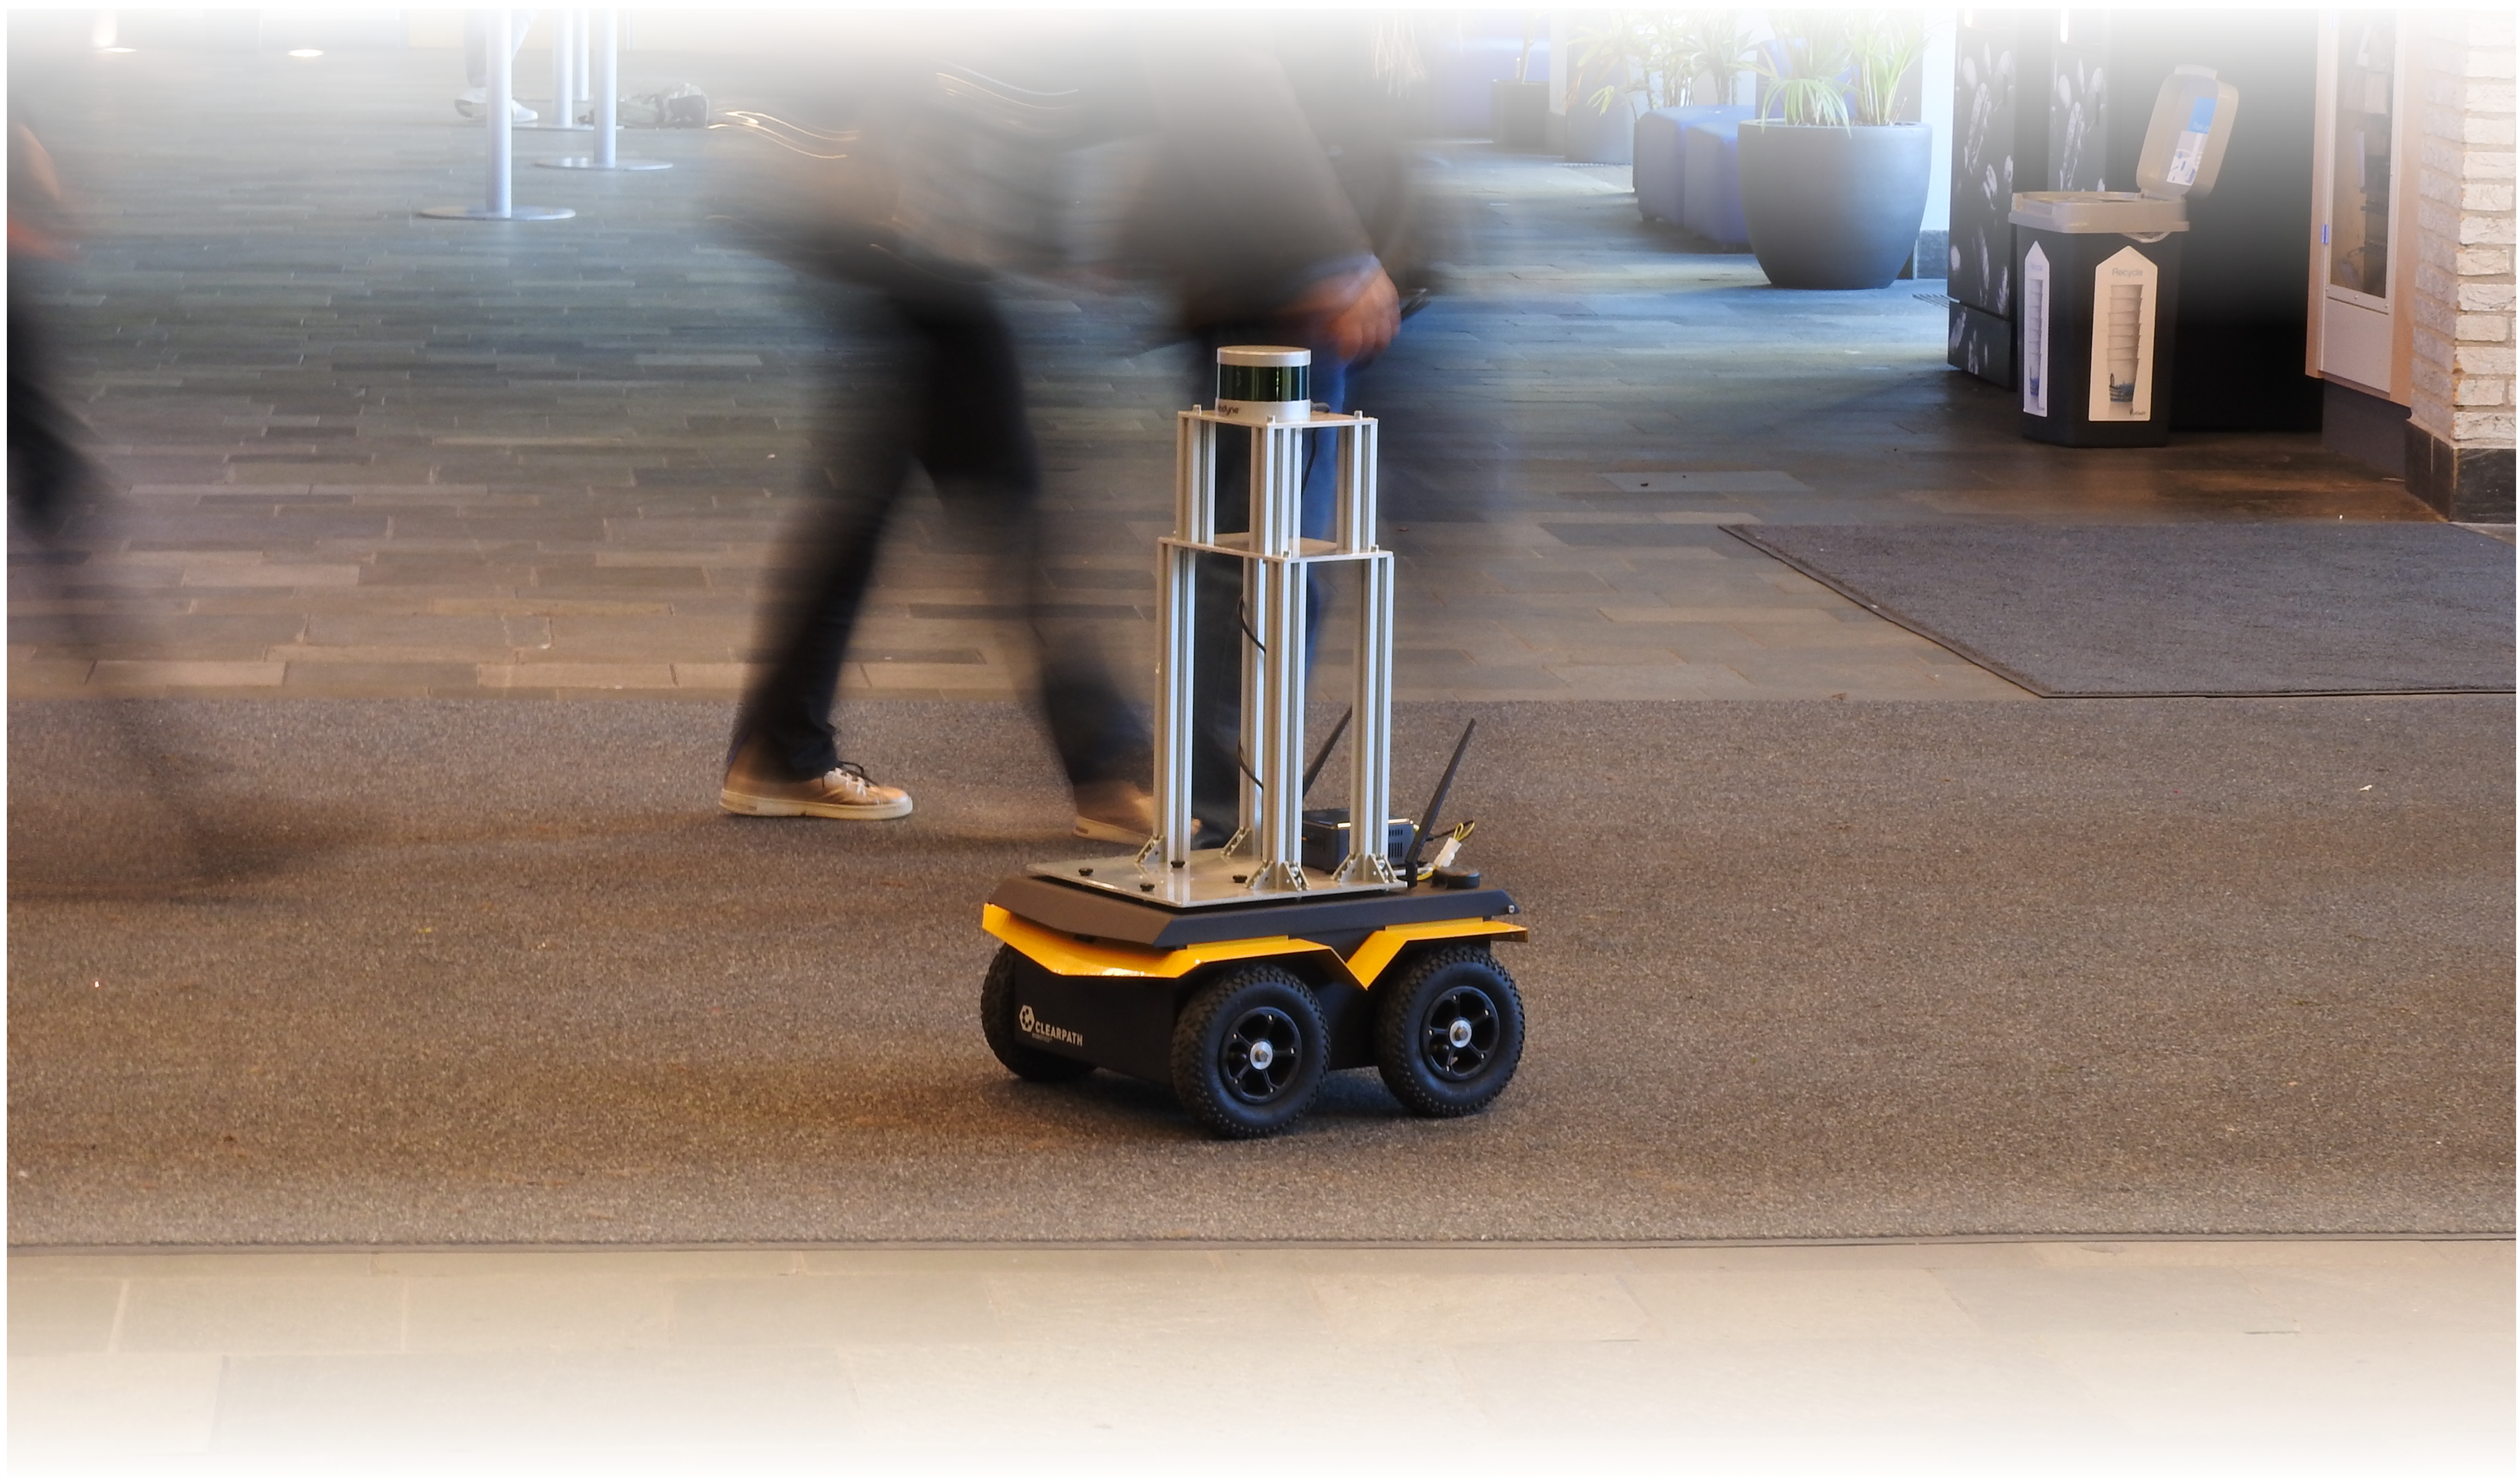
\includegraphics[width=.9\textwidth]{figs/cover.pdf} 
\caption{\emph{S3: experimental results with a pedestrian dummy.} Commanded acceleration, steering wheel angle, and longitudinal velocity of the vehicle.}
\label{fig:experiments}   
\end{figure*} 

\textbf{Month 1-4}The project will beginning with the definition of a set of experiments targeting to record data with scenarios where a mobile robot platform navigates in the same environment as other pedestrians. I will use the Jackal mobile platform presented in Fig. \ref{}.

\textbf{Month 5-8}

\textbf{Month 9-12}

\textbf{Year 3-4}

\section{The strength of the student for achieving the proposal milestones}\label{student}

The proposed research project brings together the fields of robotics, motion planning and machine learning. I have a master in electrical and computers engineering with a major in robotics. Afterwards, I did a 2 years traineeship in the Guidance, Navigation and Control (GNC) section at the European Space Agency (ESA). Here,

%% references
\\
\bibliographystyle{elsarticle-harv} 
\bibliography{ref}


%% appendix

% \section*{Appendix}
% research tree


\end{document}
